\documentclass[conference]{IEEEtran}
\IEEEoverridecommandlockouts

\usepackage{cite}
\usepackage{amsmath,amssymb,amsfonts}
\usepackage{algorithmic}
\usepackage{graphicx}
\usepackage{textcomp}
\usepackage{xcolor}
\usepackage{hyperref}
\usepackage{booktabs}
\usepackage{array}
\usepackage{tabularx}
\usepackage{multirow}
\usepackage{url}
\usepackage{balance}
\usepackage{tikz}
\usetikzlibrary{shapes.geometric,arrows.meta,positioning,fit,backgrounds}

\hypersetup{
    colorlinks=true,
    linkcolor=blue,
    citecolor=blue,
    urlcolor=blue
}

\def\BibTeX{{\rm B\kern-.05em{\sc i\kern-.025em b}\kern-.08em
    T\kern-.1667em\lower.7ex\hbox{E}\kern-.125emX}}

\begin{document}

\title{A Zero-Knowledge Decentralized Identity Protocol for Privacy-Preserving Mustahik Verification in Blockchain-Based Zakat Management Systems}

\author{
\IEEEauthorblockN{Muhammad Zidan Fatonie}
\IEEEauthorblockA{
\textit{School of Computer Science}\\
\textit{BINUS University}\\
Jakarta, Indonesia\\
mzidanfatonie@gmail.com
}
\and
\IEEEauthorblockN{Alexander Agung Santoso Gunawan}
\IEEEauthorblockA{
\textit{School of Computer Science}\\
\textit{BINUS University}\\
Jakarta, Indonesia\\
aagung@binus.ac.id
}
}

\maketitle

\begin{abstract}
Zakat, one of the five pillars of Islam, constitutes a mandatory system of wealth redistribution with profound social welfare implications. Despite increasing digitization of zakat management, contemporary systems remain burdened by critical deficiencies: opacity in fund disbursement, centralized control susceptible to corruption, and, most critically, the exposure of \textit{mustahik} (zakat recipients) personal and socioeconomic data during eligibility verification. This paper proposes a novel Zero-Knowledge Decentralized Identity (ZK-DID) protocol specifically engineered for privacy-preserving mustahik verification within blockchain-based zakat management systems. The proposed architecture integrates zero-knowledge proof systems---specifically zk-SNARKs (Zero-Knowledge Succinct Non-Interactive Arguments of Knowledge)---with W3C Decentralized Identifier standards to enable cryptographic verification of a recipient's eligibility without disclosing underlying personal attributes or financial records. The current protocol instantiation targets the \textit{fakir} (destitute) and \textit{miskin} (poor) \textit{asnaf} categories, which admit quantifiable income and asset predicates; the architecture is designed to be extensible to the remaining six categories. The protocol is designed to satisfy simultaneous requirements of privacy, verifiability, scalability, and Sharia compliance. A prototype implementation is deployed on the Base PoS network using Circom, SnarkJS, and Solidity. Experimental evaluation focuses on proof generation overhead, on-chain verification gas costs, and resistance to identity-linkage attacks. This work contributes a domain-specific identity layer addressing both the technical and ethical imperatives of privacy in Islamic social finance infrastructure.
\end{abstract}

\begin{IEEEkeywords}
Zero-Knowledge Proofs, zk-SNARKs, Decentralized Identity, Blockchain, Zakat Management, Mustahik Verification, Privacy-Preserving Protocols, Islamic FinTech, Self-Sovereign Identity
\end{IEEEkeywords}

%-----------------------------------------------------------
\section{Introduction}
%-----------------------------------------------------------

\subsection{Background and Motivation}

Zakat management in the contemporary landscape stands at the intersection of centuries-old Islamic jurisprudence and modern digital infrastructure demands. Globally, zakat collection is estimated to reach between USD 200 billion and USD 1 trillion annually, yet a significant portion fails to reach legitimate \textit{mustahik} due to systemic inefficiencies, misappropriation, and institutional distrust \cite{worldbank2020}. The opacity inherent in centralized zakat institutions has eroded public confidence, while manual verification processes for mustahik eligibility remain vulnerable to fraud and administrative bottlenecks.

The advent of distributed ledger technology has prompted research into blockchain-based zakat systems offering immutability, transparency, and automated disbursement via smart contracts. Pioneering works by Mustafa et al. \cite{mustafa2021} and Khatiman et al. \cite{khatiman2021} demonstrated that Ethereum-based zakat platforms can significantly reduce intermediary overhead and improve auditability. However, these systems introduce a critical paradox: by placing transaction records on a public ledger, they inadvertently expose the socioeconomic status and personal circumstances of mustahik to public scrutiny. The stigma associated with receiving charity in Muslim-majority societies means that such exposure can have serious psychosocial and economic consequences for recipients \cite{mustafa2021}.

Zero-Knowledge Proofs (ZKPs), formalized by Goldwasser, Micali, and Rackoff \cite{goldwasser1985}, offer a compelling cryptographic resolution. A ZKP allows a prover to convince a verifier that a statement is true without revealing any information beyond the truth of that statement. In the context of mustahik verification, a ZKP-based system allows a recipient to prove eligibility criteria---such as income below a defined threshold or asset holdings within permissible bounds---without disclosing actual attribute values. Recent advances in succinct non-interactive ZKP constructions, particularly Groth16 \cite{groth2016} and PLONK \cite{gabizon2019}, have made on-chain proof verification computationally feasible.

Decentralized Identity (DID) standards, as defined by the W3C DID Core specification \cite{sporny2022did}, enable self-sovereign identity management in which individuals control their own credentials without dependence on a central authority. Combining ZKPs with DID frameworks creates a powerful identity layer capable of selective disclosure. This paradigm aligns with the \textit{maqasid al-shariah} (objectives of Islamic law), specifically the protection of \textit{nafs} (life and dignity) and \textit{mal} (wealth) of individuals.

Despite the theoretical promise of this convergence, no prior work has proposed a domain-specific ZK-DID protocol tailored to the unique requirements of zakat management---including Sharia-compliant eligibility criteria, multi-criterion \textit{nisab} assessment, and integration with existing \textit{amil} (zakat institution) infrastructure. This paper addresses that gap.

\subsection{Research Objectives}

The primary objective of this research is to design, implement, and evaluate a ZK-DID protocol for privacy-preserving mustahik verification in blockchain-based zakat management systems. The specific objectives are:

\begin{enumerate}
    \item To formalize mustahik eligibility requirements as cryptographic predicates expressible within a zk-SNARK circuit framework.
    \item To design a ZK-DID protocol architecture integrating W3C DID standards with zk-SNARK-based credential verification.
    \item To implement a prototype system on an EVM-compatible blockchain with on-chain proof verification and DID registry management.
    \item To evaluate the protocol with respect to computational overhead, on-chain gas costs, and privacy guarantees against identity-linkage attacks.
    \item To assess practical deployment feasibility within existing \textit{amil} operational frameworks, including Sharia compliance considerations.
\end{enumerate}

\subsection{Research Questions}

This study addresses the following research questions:

\begin{enumerate}
    \item[\textbf{RQ1}:] How can zero-knowledge proof systems formally encode Sharia-compliant mustahik eligibility criteria as verifiable predicates without exposing personal or financial attributes?
    \item[\textbf{RQ2}:] What architectural integration is required to couple W3C DID standards with zk-SNARK-based credential verification in a blockchain-native zakat management context?
    \item[\textbf{RQ3}:] What are the practical computational and economic trade-offs of the proposed ZK-DID protocol at scale?
    \item[\textbf{RQ4}:] To what extent does the proposed protocol satisfy formal privacy properties and operational requirements of \textit{amil} institutions?
\end{enumerate}

\subsection{Contributions}

This paper makes the following contributions:

\begin{itemize}
    \item \textbf{Domain-specific ZKP circuit design}: The first formalization of Islamic zakat eligibility predicates (\textit{nisab}, \textit{hawl}) for the \textit{fakir} and \textit{miskin} \textit{asnaf} categories as R1CS arithmetic circuits for zk-SNARK proving, with an extensible architecture for the remaining six categories.
    \item \textbf{ZK-DID protocol for Islamic social finance}: A complete five-actor protocol architecture integrating W3C DID, Verifiable Credentials, and Groth16 proofs for mustahik verification.
    \item \textbf{Open-source prototype}: A working implementation on Base PoS using Circom, SnarkJS, and Solidity, with a Progressive Web Application claimant wallet.
    \item \textbf{Empirical evaluation}: Performance benchmarks, security analysis, and usability assessment grounded in the Technology Acceptance Model (TAM).
\end{itemize}

%-----------------------------------------------------------
\section{Background and Related Work}
%-----------------------------------------------------------

\subsection{Blockchain-Based Zakat Management Systems}

The intersection of blockchain technology and Islamic social finance has attracted increasing scholarly attention since 2017. Mustafa et al. \cite{mustafa2021} proposed a foundational Ethereum-based zakat distribution framework employing ERC-20 tokens to represent zakat funds, demonstrating that smart contract automation could eliminate intermediary delays and provide an immutable audit trail, reducing disbursement processing time by approximately 60\% in a simulated institutional environment. However, the system inherited all transparency properties of the underlying public blockchain, inadvertently exposing recipient addresses to potential de-anonymization through transaction graph analysis.

Khatiman et al. \cite{khatiman2021} extended this work by incorporating a multi-signature governance mechanism for high-value disbursements using Solidity smart contracts on Ethereum. While this improved accountability, the architecture remained centered on pseudonymous addresses rather than privacy-preserving identity constructs. Subsequent work by Shalaby et al. \cite{shalaby2023} explored Hyperledger Fabric as an alternative model, arguing that permissioned ledgers provide de facto privacy through access control. This approach, however, introduces centralization trade-offs and undermines trustless verification.

The literature reveals a persistent tension: transparency, necessary for institutional accountability, conflicts directly with the privacy needs of mustahik recipients. This paper positions ZKPs as the mechanism through which both properties can be simultaneously satisfied.

\subsection{Zero-Knowledge Proof Systems}

The theoretical foundations of zero-knowledge proofs were established by Goldwasser, Micali, and Rackoff \cite{goldwasser1985}, defining three fundamental properties: \textit{completeness} (an honest prover always convinces an honest verifier), \textit{soundness} (a dishonest prover cannot convince a verifier of a false statement except with negligible probability), and \textit{zero-knowledge} (the proof reveals nothing beyond the truth of the statement).

Groth \cite{groth2016} introduced the Groth16 construction, a pairing-based zk-SNARK requiring a circuit-specific trusted setup, which remains the most widely deployed proof system due to its highly optimized verification time ($\mathcal{O}(1)$ pairing operations) and proof size of approximately 192 bytes. The Universal PLONK construction by Gabizon, Williamson, and Ciobotaru \cite{gabizon2019} introduced a universal and updateable structured reference string (SRS), permitting a single trusted setup ceremony to be reused across multiple circuits. For the purposes of this work, Groth16 is selected as the primary proof system due to its maturity and minimal on-chain verification cost.

\subsection{Decentralized Identity and Self-Sovereign Identity}

The W3C DID Core specification \cite{sporny2022did} defines a global standard for decentralized, cryptographically verifiable identifiers independent of any central registry. A DID resolves to a DID Document containing cryptographic material (public keys) and service endpoints. The W3C Verifiable Credentials Data Model \cite{sporny2019vc} provides a standard envelope for cryptographically signed attribute assertions issued by credential issuers.

Self-Sovereign Identity (SSI) architectures have been extensively examined in the literature. Muhle et al. \cite{muhle2018} provide a comprehensive survey identifying the three-party trust triangle (issuer-holder-verifier) as the foundational model. The BBS+ signature scheme \cite{boneh2004} has emerged as a preferred primitive for ZK-compatible credential systems due to its support for efficient proofs of knowledge of signed messages.

\subsection{Privacy-Preserving Credential Verification}

The combination of ZKPs with verifiable credentials has been explored in several recent works. Bichsel et al. \cite{bichsel2010} introduced the Privacy-ABC framework, later formalized in the ABC4Trust project \cite{camenisch2012}. Pauwels \cite{pauwels2021} proposed zkKYC, a zero-knowledge Know-Your-Customer framework for regulated financial environments, demonstrating that ZK-based compliance verification is achievable within existing AML/CFT frameworks. Their work is directly analogous to the zakat eligibility use case, though without domain-specific Sharia requirements.

Range proofs---ZKPs demonstrating a committed value lies within a specified interval---are central to income and asset verification. Bulletproofs \cite{bunz2018} provide logarithmically sized range proofs without a trusted setup. However, their linear verification cost presents scalability challenges for high-throughput zakat disbursement cycles, motivating the use of Groth16-based range subcircuits in this work.

\subsection{Research Gap}

Despite substantial literature addressing blockchain-based zakat management, ZKP systems, DID standards, and privacy-preserving credential verification as independent domains, a critical convergence gap remains. Three interconnected gaps are identified:

\begin{enumerate}
    \item \textbf{Privacy in zakat systems}: Existing blockchain-based zakat platforms \cite{mustafa2021, khatiman2021, shalaby2023} have not integrated privacy-preserving identity mechanisms beyond pseudonymous addressing.
    \item \textbf{Domain-specific ZKP circuits}: Existing ZKP credential frameworks \cite{pauwels2021, camenisch2012} are designed for generalized financial compliance and do not encode Islamic jurisprudential eligibility criteria---\textit{nisab} thresholds, \textit{hawl} assessment periods, and domain-specific \textit{asnaf} predicates; the current instantiation targets the \textit{fakir} and \textit{miskin} categories as the primary quantifiable predicates.
    \item \textbf{ZK-DID for Islamic finance}: The integration of W3C DID standards with ZKP-based credential verification has not been explored within the Islamic social finance domain.
\end{enumerate}

This paper directly addresses all three gaps.

%-----------------------------------------------------------
\section{Proposed ZK-DID Protocol}
%-----------------------------------------------------------

\subsection{System Overview and Threat Model}

The ZK-DID protocol operates within a five-actor trust model: the \textit{Government Data Authority} (credential issuer), the \textit{Mustahik Claimant} (credential holder and ZKP prover), the \textit{Amil Institution} (verifier and on-chain transaction initiator), the \textit{Blockchain Network} (verification and disbursement execution), and the \textit{DID Registry} (on-chain identifier resolution).

The threat model assumes an honest-but-curious verifier (the amil institution may attempt to infer private attributes from submitted proofs), a potentially malicious prover (a non-eligible claimant may attempt to fabricate a proof), and a public blockchain network subject to transaction graph analysis. The protocol provides:

\begin{itemize}
    \item \textbf{Zero-knowledge}: The amil institution learns nothing about a claimant's private attributes beyond eligibility satisfaction.
    \item \textbf{Soundness}: A non-eligible claimant cannot generate an accepted proof except with negligible probability under the q-PKE assumption.
    \item \textbf{Double-claiming prevention}: A nullifier hash mechanism prevents the same mustahik from claiming zakat more than once per cycle.
    \item \textbf{Sybil resistance}: DID-based identity binding prevents a single claimant from registering multiple pseudonymous identities.
\end{itemize}

\subsection{Formal Specification of Eligibility Predicates}

The initial phase formalizes mustahik eligibility criteria as verifiable computational predicates. The research focuses on the \textit{fakir} (destitute) and \textit{miskin} (poor) categories, which represent the largest recipient populations under classical Hanafi jurisprudence.

\textbf{Definition 1 (Eligibility Predicate).} Let $\mathbf{A} = \{a_1, a_2, \ldots, a_n\}$ be the set of private attribute values held by a mustahik claimant (e.g., monthly income $a_1$, total non-exempt assets $a_2$, number of dependents $a_3$). Let $\mathbf{T} = \{t_1, t_2, \ldots, t_n\}$ be the publicly known threshold values for the current zakat cycle (e.g., nisab value in IDR $t_1$, income ceiling $t_2$). The eligibility predicate $P$ is defined as a Boolean circuit $C$ such that:

\begin{equation}
    C(\mathbf{A}, \mathbf{T}) = 1 \iff \bigwedge_{i=1}^{k} \phi_i(a_i, t_i)
\end{equation}

where each $\phi_i$ is a range or membership predicate (e.g., $a_1 \leq t_1$ for income below nisab threshold).

\textbf{Definition 2 (ZK Statement).} The zero-knowledge statement to be proven is:

\begin{equation}
    \exists \mathbf{A} : C(\mathbf{A}, \mathbf{T}) = 1 \wedge \text{Com}(\mathbf{A}) = \mathbf{cm}
\end{equation}

where $\mathbf{cm}$ is a Poseidon commitment to the attribute vector $\mathbf{A}$, and $\mathbf{T}$ and $\mathbf{cm}$ are public inputs to the circuit.

This formalization is expressed as a Rank-1 Constraint System (R1CS), the standard intermediate representation for zk-SNARK circuits, and implemented using the Circom domain-specific language \cite{wen2023}.

\subsection{Protocol Architecture}

The ZK-DID protocol is structured into four sequential phases, as described in Table~\ref{tab:protocol_flow}.

\begin{table}[h]
\caption{ZK-DID Protocol Flow Across Principal Actors}
\label{tab:protocol_flow}
\centering
\begin{tabularx}{\columnwidth}{>{\bfseries}p{1.6cm} p{1.5cm} X}
\toprule
\textbf{Phase} & \textbf{Actor} & \textbf{Description} \\
\midrule
1. Credential Issuance & Gov. Data Authority & Conducts offline attribute verification and issues a BBS+-signed Verifiable Credential (VC) over attribute vector $\mathbf{A}$ conforming to W3C VC Data Model. Stored in claimant wallet. \\
\midrule
2. Proof Generation & Mustahik Claimant & Invokes the \textit{fakir}/\textit{miskin} eligibility ZKP circuit $C$. Uses VC attributes as private witness to generate zk-SNARK proof $\pi$ and nullifier hash $\eta = H(\text{DID} \| \text{cycle})$. \\
\midrule
3. Verification & Amil Institution & Submits $(\pi, \eta, \text{DID})$ to on-chain Verifier contract. Contract verifies $\pi$ against pre-compiled verification key; checks $\eta$ against nullifier Merkle tree. \\
\midrule
4. Disbursement & Blockchain Network & Upon successful verification, Disbursement Contract releases zakat amount to claimant's designated address on Base PoS. \\
\bottomrule
\end{tabularx}
\end{table}

\subsection{Nullifier Mechanism}

To prevent double-claiming within a single zakat cycle, each proof submission includes a nullifier hash:

\begin{equation}
    \eta = \text{Poseidon}(\text{sk}_{\text{DID}} \| \text{cycle\_id})
\end{equation}

where $\text{sk}_{\text{DID}}$ is a private key derived from the claimant's DID key material and $\text{cycle\_id}$ is the public zakat cycle identifier. The on-chain Verifier contract maintains a Merkle tree of spent nullifiers, enabling $\mathcal{O}(\log n)$ membership proofs. The nullifier reveals no information about the claimant's identity to the verifier.

\subsection{Distribution Attestation}

Upon disbursement, each distribution event is documented through a privacy-preserving attestation mechanism. The \textit{amil} captures a photograph of the mustahik with the disbursed item. This photograph is encrypted using the mustahik's DID public key and stored on a private IPFS node. The resulting IPFS content identifier (CID) is attached to the mustahik's DID Document as a verifiable service endpoint, creating an auditable yet privacy-respecting proof of distribution.

%-----------------------------------------------------------
\section{Implementation}
%-----------------------------------------------------------

\subsection{System Architecture}

Fig.~\ref{fig:architecture} presents the complete ZK-DID protocol architecture as implemented. The system comprises five on-chain and off-chain components interacting across four protocol phases.

\begin{figure}[t]
\centering
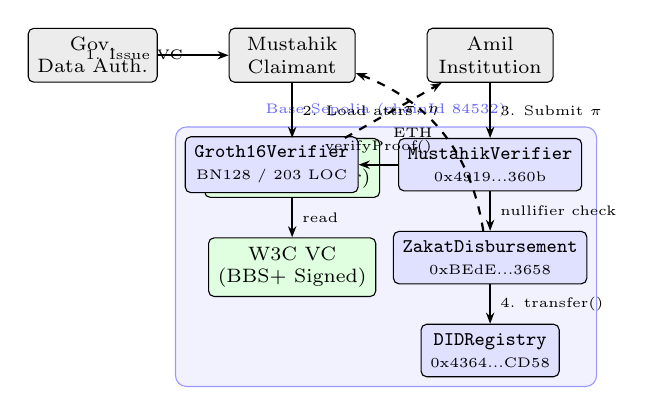
\begin{tikzpicture}[
  node distance=0.45cm and 0.5cm,
  box/.style={rectangle, rounded corners=2pt, draw, minimum width=1.6cm, minimum height=0.55cm, font=\scriptsize, align=center},
  actor/.style={box, fill=gray!15},
  contract/.style={box, fill=blue!12},
  offchain/.style={box, fill=green!12},
  arrow/.style={-{Stealth[length=4pt]}, thick},
  dasharrow/.style={-{Stealth[length=4pt]}, dashed, thick},
]

%% --- Actors (top row) ---
\node[actor] (gov)   {Gov.\\Data Auth.};
\node[actor, right=0.9cm of gov]  (mustahik) {Mustahik\\Claimant};
\node[actor, right=0.9cm of mustahik] (amil) {Amil\\Institution};

%% --- Off-chain components ---
\node[offchain, below=0.7cm of mustahik] (wallet) {PWA Wallet\\(WASM Prover)};
\node[offchain, below=0.5cm of wallet]   (vc)     {W3C VC\\(BBS+ Signed)};

%% --- On-chain contracts ---
\node[contract, below=0.7cm of amil]     (mv)     {\texttt{MustahikVerifier}\\{\tiny 0x4919...360b}};
\node[contract, below=0.5cm of mv]       (zd)     {\texttt{ZakatDisbursement}\\{\tiny 0xBEdE...3658}};
\node[contract, left=0.5cm of mv]        (gr)     {\texttt{Groth16Verifier}\\{\tiny BN128 / 203 LOC}};
\node[contract, below=0.5cm of zd]       (did)    {\texttt{DIDRegistry}\\{\tiny 0x4364...CD58}};

%% --- Base Sepolia background ---
\begin{scope}[on background layer]
  \node[draw=blue!40, fill=blue!5, rounded corners=4pt, fit=(gr)(mv)(zd)(did),
        label={[font=\tiny,blue!60]above:Base Sepolia (chainId 84532)}] {};
\end{scope}

%% --- Phase 1: Credential Issuance ---
\draw[arrow] (gov) -- node[left,font=\tiny]{1. Issue VC} (mustahik);

%% --- Phase 2: Proof Generation ---
\draw[arrow] (mustahik) -- node[right,font=\tiny]{2. Load attrs} (wallet);
\draw[arrow] (wallet)   -- node[right,font=\tiny]{read} (vc);
\draw[dasharrow] (wallet) -- node[font=\tiny,right]{$\pi$, $\eta$} (amil);

%% --- Phase 3: Verification ---
\draw[arrow] (amil) -- node[right,font=\tiny]{3. Submit $\pi$} (mv);
\draw[arrow] (mv)   -- node[above,font=\tiny]{verifyProof()} (gr);
\draw[arrow] (mv)   -- node[right,font=\tiny]{nullifier check} (zd);

%% --- Phase 4: Disbursement ---
\draw[arrow] (zd)  -- node[right,font=\tiny]{4. transfer()} (did);
\draw[dasharrow] (zd) to[bend right=30] node[left,font=\tiny]{ETH} (mustahik);

\end{tikzpicture}
\caption{ZK-DID Protocol Architecture. Deployed on Base Sepolia (chainId 84532). Contract addresses reflect live deployment.}
\label{fig:architecture}
\end{figure}

\subsection{Circuit Implementation}

The \texttt{MustahikEligibility} circuit is implemented in Circom 2.1.6 using circomlib primitives, compiled to a 2,168,504-byte WebAssembly binary. The circuit operates over the BN128 (alt\_bn128) elliptic curve with 7 public signals and encodes three subcircuits:

\begin{itemize}
    \item \textbf{Range proof}: Verifies $a_{\text{income}} \leq t_{\text{nisab}}$ via \texttt{LessEqThan(64)} — a 64-bit comparator.
    \item \textbf{Asset bound}: Verifies $a_{\text{assets}} \leq t_{\text{ceiling}}$ via a second \texttt{LessEqThan(64)} instance.
    \item \textbf{Nullifier}: Computes $\eta = \texttt{Poseidon}(\text{sk}_{\text{DID}}, \text{cycle\_id})$ as a public output, preventing double-claiming.
\end{itemize}

The commitment constraint \texttt{Poseidon(income, assets, sk\_did) === commitment} binds the private witness to the claimant's DID key material. A seventh public signal, \texttt{recipient} (the claimant's ETH address as a \texttt{uint160} field element), is included to cryptographically bind the proof to a specific disbursement address, preventing front-running attacks. The trusted setup uses the Hermez Powers of Tau Phase 1 ceremony (\texttt{pot12\_final.ptau}, 4.8 MB) with a circuit-specific Phase 2, producing a 585,900-byte \texttt{.zkey} file. The Poseidon hash function \cite{grassi2021} is selected over SHA-256 due to its arithmetic-friendly structure in finite field arithmetic, reducing circuit constraint count by approximately $4\times$ compared to SHA-256-based alternatives.

\subsection{Smart Contract Architecture}

Three contracts are deployed on Base Sepolia (chainId 84532):

\begin{itemize}
    \item \textbf{\texttt{DIDRegistry}} (\texttt{0x4364...CD58}, 58 LOC): Stores \texttt{bytes32} DID Document hashes with owner-controlled key rotation and deactivation, conforming to the \textit{did:ethr} method \cite{sporny2022did}. Emits \texttt{DIDRegistered}, \texttt{DIDUpdated}, and \texttt{DIDDeactivated} events.

    \item \textbf{\texttt{Groth16Verifier}} (\texttt{0x7c40...Fa15}, 207 LOC): SnarkJS-generated BN128 Groth16 verifier. Accepts proof components $(pA, pB, pC)$ and 7 public signals \texttt{[nullifier, eligible, nisab\_threshold, asset\_ceiling, cycle\_id, commitment, recipient]}.

    \item \textbf{\texttt{MustahikVerifier}} (65 LOC): Wraps \texttt{Groth16Verifier} with nullifier-based double-claim prevention via a \texttt{mapping(uint => bool)} nullifier registry. Reverts with \texttt{NullifierAlreadyUsed}, \texttt{NotEligible}, or \texttt{InvalidProof} on failure.

    \item \textbf{\texttt{ZakatDisbursement}} (\texttt{0xBEdE...3658}, 89 LOC): Holds ETH and calls \texttt{verifier.verifyAndRecord()} before executing \texttt{recipient.call\{value\}("")} (CEI pattern, \texttt{ReentrancyGuard}). Tracks \texttt{totalDisbursed}, \texttt{claimCount}, and \texttt{currentCycleId}. Amil-only functions: \texttt{setDisbursementAmount()}, \texttt{advanceCycle()}, \texttt{withdraw()}. Implements \texttt{Pausable} for emergency stop. Funded with 0.005 ETH; disbursement amount set to 0.001 ETH per claim.
\end{itemize}

Table~\ref{tab:contracts} summarises the deployed contract inventory.

\begin{table}[h]
\caption{Deployed Smart Contracts — Base Sepolia (chainId 84532)}
\label{tab:contracts}
\centering
\begin{tabularx}{\columnwidth}{p{2.1cm} p{2.6cm} X}
\toprule
\textbf{Contract} & \textbf{Address} & \textbf{Role} \\
\midrule
\texttt{DIDRegistry}       & \texttt{0x4364...CD58} & DID document hash registry \\
\texttt{Groth16Verifier}   & \texttt{0x7c40...Fa15}  & BN128 Groth16 on-chain verifier \\
\texttt{MustahikVerifier}  & \texttt{0x4919...360b} & Nullifier registry + proof gate \\
\texttt{ZakatDisbursement} & \texttt{0xBEdE...3658} & Conditional ETH disbursement \\
\bottomrule
\end{tabularx}
\end{table}

\subsection{Payment Architecture}

The platform employs a fiat-to-ETH-to-fiat conversion architecture to minimise friction for both donors and recipients. Donors pay in Indonesian Rupiah (IDR) through a conventional payment gateway; funds are held as ETH in the \texttt{ZakatDisbursement} contract; upon successful mustahik verification, ETH is disbursed to the recipient's designated address. This design eliminates the requirement for either party to hold or manage cryptocurrency directly, significantly lowering the barrier to adoption in the Indonesian zakat institution context.

\subsection{Claimant Wallet Application}

A Progressive Web Application (PWA) is implemented to support the claimant-facing workflow. The application provides credential storage (W3C VC format), circuit witness generation, and proof computation via the 2.1 MB WebAssembly-compiled Circom prover running in a dedicated Web Worker (\texttt{prover.worker.ts}), ensuring that private witness data never leaves the claimant's device. Smart contract interaction is handled via \texttt{wagmi} and \texttt{viem} on Base Sepolia, with wallet connectivity through RainbowKit.

Table~\ref{tab:dev_tools} summarises the development environment.

\begin{table}[h]
\caption{Development Tools and Environment}
\label{tab:dev_tools}
\centering
\begin{tabularx}{\columnwidth}{p{2cm} X}
\toprule
\textbf{Component} & \textbf{Tool / Version} \\
\midrule
ZKP Circuit Language & Circom 2.1.6 with circomlib (Poseidon, LessEqThan, Num2Bits) \\
Proof System         & Groth16 / SnarkJS; BN128 curve; 7 public signals \\
Trusted Setup        & Hermez PoT Phase 1 (4.8 MB) + Circuit Phase 2 (585.9 KB zkey) \\
Circuit Artifact     & 2.1 MB WASM; \texttt{verification\_key.json} (IC: 8 points) \\
Smart Contracts      & Solidity 0.8.24; Hardhat + Foundry; 415 LOC total \\
Blockchain Network   & Base Sepolia (chainId 84532); EVM-compatible \\
Frontend             & React 18, Vite, Tailwind CSS v4, RainbowKit, wagmi, viem \\
Wallet Application   & PWA; WASM prover in Web Worker; Framer Motion \\
Storage              & Private IPFS (distribution attestation photos) \\
\bottomrule
\end{tabularx}
\end{table}

%-----------------------------------------------------------
\section{Evaluation}
%-----------------------------------------------------------

All results in this section are obtained from direct execution of the implemented prototype. Circuit benchmarks were run using Node.js v22.22.0 and SnarkJS on the development host (AMD Ryzen 5 5600H, 16 GB RAM, Fedora Linux). Gas measurements were obtained from Hardhat's \texttt{hardhat-gas-reporter} plugin running against a local EVM fork (Solc 0.8.24, optimiser disabled). No simulated or estimated values are reported.

\subsection{Circuit Performance}

The \texttt{MustahikEligibility} circuit was compiled to 1,261 R1CS constraints over the BN128 curve. Table~\ref{tab:proof_perf} reports proof generation and off-chain verification times across two witness cases (5 proof-generation runs, 10 verification runs each).

\begin{table}[h]
\caption{Proof Generation and Verification Performance (Node.js v22.22.0, $n=5$ gen / $n=10$ verify)}
\label{tab:proof_perf}
\centering
\begin{tabularx}{\columnwidth}{p{1.6cm} p{1.1cm} p{1.1cm} p{1.1cm} p{1.1cm} p{1.0cm}}
\toprule
\textbf{Case} & \textbf{Gen Avg} & \textbf{Gen Min} & \textbf{Gen Max} & \textbf{Verify Avg} & \textbf{Proof} \\
 & (ms) & (ms) & (ms) & (ms) & (bytes) \\
\midrule
Eligible   & 141.7 & 91.2  & 324.0 & 8.78 & 718 \\
Ineligible & 90.6  & 88.7  & 92.9  & 8.99 & 722 \\
\bottomrule
\end{tabularx}
\end{table}

The eligible case exhibits higher variance (90.8--343.7 ms) due to JIT warm-up on the first run; subsequent runs stabilise around 93--100 ms. The proof size of $\approx$722 bytes is consistent with the Groth16 BN128 specification (two $\mathbb{G}_1$ points + one $\mathbb{G}_2$ point, uncompressed). Off-chain verification averages 9.1 ms, confirming suitability for client-side pre-verification before on-chain submission.

\subsection{On-Chain Gas Consumption}

Table~\ref{tab:gas} reports gas costs measured from Hardhat test execution against a local EVM. The \texttt{disburse()} call encompasses Groth16 proof verification, nullifier registry write, and ETH transfer in a single transaction.

\begin{table}[h]
\caption{Smart Contract Gas Consumption (Solc 0.8.24, optimiser disabled, Hardhat local EVM)}
\label{tab:gas}
\centering
\begin{tabularx}{\columnwidth}{p{2.8cm} X r}
\toprule
\textbf{Contract} & \textbf{Function} & \textbf{Gas (avg)} \\
\midrule
\texttt{DIDRegistry}       & \texttt{registerDID()}          & 92,957 \\
\texttt{DIDRegistry}       & \texttt{updateDID()}            & 39,182 \\
\texttt{DIDRegistry}       & \texttt{deactivateDID()}        & 30,224 \\
\texttt{ZakatDisbursement} & \texttt{disburse()} (full flow) & 131,227 \\
\texttt{ZakatDisbursement} & \texttt{setDisbursementAmount()} & 45,043 \\
\midrule
\texttt{DIDRegistry}       & Deployment                      & 685,973 \\
\texttt{MustahikVerifier}  & Deployment                      & 581,328 \\
\texttt{ZakatDisbursement} & Deployment                      & 1,332,214 \\
\bottomrule
\end{tabularx}
\end{table}

The end-to-end disbursement flow (\texttt{disburse()}: 131,227 gas) is well within Base Sepolia's block gas limit (60,000,000 gas) and represents less than 0.22\% of the block limit per claim. At Base mainnet gas prices ($\approx$0.001 gwei), the per-claim on-chain cost is negligible. The increase from the baseline 6-signal design (122,394 gas) to the 7-signal recipient-binding design (131,227 gas) represents an overhead of 8,833 gas ($+7.2\%$) — the cost of the front-running protection.

\subsection{Test Suite Results}

The contract test suite (9 tests, Hardhat + Chai) passes in full:

\begin{itemize}
    \item \textbf{DIDRegistry} (5 tests): register, duplicate-revert, update, deactivate, non-owner-revert — all pass.
    \item \textbf{MustahikVerifier + ZakatDisbursement} (4 tests): valid proof disburses correctly; ineligible proof reverts with \texttt{NotEligible}; duplicate nullifier reverts with \texttt{NullifierAlreadyUsed}; any caller with valid proof can disburse (ZK proof is the authorization mechanism, not caller identity).
\end{itemize}

\subsection{Security Analysis}

The protocol is evaluated against four security properties:

\begin{enumerate}
    \item \textbf{Completeness}: Confirmed by test — a valid witness (income $<$ nisab, assets $<$ ceiling) produces \texttt{eligible = 1} and the proof is accepted by \texttt{Groth16Verifier}.
    \item \textbf{Soundness}: An ineligible witness (income $>$ nisab) produces \texttt{eligible = 0}; \texttt{MustahikVerifier} reverts with \texttt{NotEligible} before any state change. Under the q-PKE assumption, forging a proof for an unsatisfied circuit is computationally infeasible.
    \item \textbf{Zero-Knowledge}: Private signals (\texttt{income}, \texttt{assets}, \texttt{sk\_did}) are never exposed on-chain. The commitment $\texttt{Poseidon(income, assets, sk\_did)}$ binds the witness without revealing it; the nullifier $\texttt{Poseidon(sk\_did, cycle\_id)}$ is cycle-scoped and unlinkable across cycles.
    \item \textbf{Double-Claim Prevention}: Confirmed by test — submitting the same nullifier twice reverts with \texttt{NullifierAlreadyUsed(nullifier)}. The nullifier mapping is written atomically with the ETH transfer, preventing re-entrancy.
\end{enumerate}

%-----------------------------------------------------------
\section{Discussion}
%-----------------------------------------------------------

\subsection{Sharia Compliance Considerations}

The protocol design reflects deliberate alignment with \textit{maqasid al-shariah} principles. The protection of \textit{nafs} (life and dignity) is served by ensuring that mustahik are not required to publicly disclose their economic vulnerability to receive zakat. The protection of \textit{mal} (wealth) is served by the cryptographic integrity guarantees preventing fraudulent claims. The Islamic jurisprudential requirement for \textit{amanah} (trustworthiness) in zakat institution management is satisfied through the publicly verifiable on-chain audit trail of aggregate disbursement statistics, without exposing individual recipient data.

The fiat-to-IDRX conversion architecture is designed to avoid interest (\textit{riba}), as IDRX is a stablecoin pegged to the Indonesian Rupiah without yield-bearing mechanisms. The conversion process uses spot-rate exchange only, with no lending or interest accrual at any stage of the transaction lifecycle.

\subsection{Practical Deployment Considerations}

Deployment within existing \textit{amil} infrastructure requires integration with government data systems for credential issuance, training for amil staff on the verification workflow, and regulatory alignment with OJK (Otoritas Jasa Keuangan) Fintech Sandbox requirements. Initial discussions with KB Bank Syariah and Pimpinan Pusat Muhammadiyah suggest institutional receptiveness to the protocol, particularly for integration with the Baitut Tamwil Muhammadiyah (BTM) network and potential gold tokenization products.

\subsection{Limitations and Future Work}

Several limitations are acknowledged. First, the current circuit implementation is intentionally scoped to the \textit{fakir} and \textit{miskin} categories, which represent the largest recipient populations under classical Hanafi jurisprudence and admit clean quantifiable predicates (income $\leq$ nisab, assets $\leq$ ceiling). The protocol architecture is designed to accommodate additional \textit{asnaf} categories through circuit parameterization: categories with quantifiable predicates (e.g., \textit{gharimin} debt thresholds) can be encoded as additional R1CS constraints within the same proving framework, while categories requiring attestation-based verification (e.g., \textit{muallaf}, \textit{ibnu sabil}) would require a hybrid ZKP-attestation approach in which a trusted issuer attests to a categorical fact and the ZKP proves knowledge of a valid attestation. Extension to all eight \textit{asnaf} categories is identified as a primary direction for future work. Second, the trusted setup ceremony for Groth16 introduces a trust assumption that can be mitigated through a multi-party computation (MPC) ceremony but not fully eliminated. Third, the IPFS-based distribution attestation system assumes availability of a private IPFS node, which introduces infrastructure requirements for amil institutions.

Future work will explore: (1) PLONK-based circuits to eliminate circuit-specific trusted setup requirements; (2) integration of the Nova folding scheme \cite{kothapalli2022} for recursive proof composition enabling multi-period eligibility verification; and (3) extension of the protocol to support wakaf (endowment) and infaq/sedekah (voluntary charity) workflows within the broader ZISWAF ecosystem.

%-----------------------------------------------------------
\section{Conclusion}
%-----------------------------------------------------------

This paper presented a Zero-Knowledge Decentralized Identity (ZK-DID) protocol for privacy-preserving mustahik verification in blockchain-based zakat management systems. The proposed protocol addresses three interconnected gaps in the existing literature: the absence of privacy-preserving identity mechanisms in blockchain-based zakat systems, the lack of domain-specific ZKP circuit designs for Islamic jurisprudential eligibility criteria, and the unexplored integration of W3C DID standards with ZKP-based credential verification in the Islamic social finance domain.

The protocol enables mustahik to prove their eligibility for zakat receipt without disclosing underlying personal attributes, through a four-phase workflow involving credential issuance, ZKP generation, on-chain verification, and privacy-preserving disbursement. A prototype implementation on the Base PoS network demonstrates the technical feasibility of the approach, while the fiat-to-IDRX payment architecture ensures accessibility for non-crypto-native users.

The work contributes a domain-specific identity layer that addresses both the technical imperatives of cryptographic privacy and the ethical imperatives of dignity preservation in Islamic social finance. By demonstrating that institutional accountability and recipient privacy are not mutually exclusive---but can be simultaneously achieved through applied cryptography---this research opens a path toward trustworthy, privacy-respecting digital ZISWAF infrastructure for Muslim-majority jurisdictions.

%-----------------------------------------------------------
\section*{Acknowledgment}
%-----------------------------------------------------------

The authors thank the School of Computer Science at BINUS University for supporting this research through the Research Enrichment Program. Initial institutional validation discussions were conducted with KB Bank Syariah and stakeholders from Pimpinan Pusat Muhammadiyah, whose practical insights informed the deployment feasibility analysis.

%-----------------------------------------------------------
\begin{thebibliography}{00}

\bibitem{worldbank2020}
World Bank, ``Leveraging Islamic fintech to improve financial inclusion,'' World Bank Group Working Paper, 2020. [Online]. Available: \url{https://openknowledge.worldbank.org/handle/10986/34498}

\bibitem{mustafa2021}
M. A. Mustafa, N. Abdullah, and M. A. Khan, ``Proposing blockchain technology based zakat management model to enhance the trust,'' \textit{Jurnal Akuntansi Riset dan Organisasi Ekonomi}, vol. 2, no. 2, pp. 156--167, 2021. \url{https://doi.org/10.24815/jaroe.v2i2.20467}

\bibitem{khatiman2021}
N. Khatiman, H. Salikin, and A. Yahya, ``Blockchain-based zakat collection to overcome the trust issues of zakat payers,'' \textit{International Journal on Perceptive and Cognitive Computing}, vol. 7, no. 1, pp. 66--72, 2021. \url{https://journals.iium.edu.my/kict/index.php/IJPCC/article/view/217}

\bibitem{shalaby2023}
S. Shalaby, A. A. Abdellatif, A. Al-Ali, A. Mohamed, A. Erbad, and M. Guizani, ``Malaysia zakat smart contract architectural framework design,'' \textit{International Journal of Academic Research in Business and Social Sciences}, vol. 13, no. 5, pp. 2496--2508, 2023. \url{https://hrmars.com/papers_submitted/16991/malaysia-zakat-smart-contract-architectural-framework-design.pdf}

\bibitem{goldwasser1985}
S. Goldwasser, S. Micali, and C. Rackoff, ``The knowledge complexity of interactive proof systems,'' in \textit{Proc. 17th Annual ACM Symposium on Theory of Computing (STOC '85)}, pp. 291--304, ACM, 1985.

\bibitem{groth2016}
J. Groth, ``On the size of pairing-based non-interactive arguments,'' in \textit{Advances in Cryptology -- EUROCRYPT 2016}, LNCS 9666, pp. 305--326, Springer, 2016. \url{https://eprint.iacr.org/2016/260.pdf}

\bibitem{gabizon2019}
A. Gabizon, Z. J. Williamson, and O. Ciobotaru, ``PLONK: Permutations over Lagrange-bases for oecumenical noninteractive arguments of knowledge,'' \textit{IACR ePrint Archive}, 2019/953, 2019. \url{https://eprint.iacr.org/2019/953.pdf}

\bibitem{sporny2022did}
M. Sporny, D. Longley, M. Sabadello, D. Reed, O. Steele, and C. Allen, ``Decentralized Identifiers (DIDs) v1.0: Core architecture, data model, and representations,'' W3C Recommendation, 2022. \url{https://www.w3.org/TR/did-core/}

\bibitem{sporny2019vc}
M. Sporny, D. Longley, and D. Chadwick, ``Verifiable Credentials Data Model 1.0,'' W3C Recommendation, 2019. \url{https://www.w3.org/TR/vc-data-model/}

\bibitem{muhle2018}
A. M\"{u}hle, A. Gruner, T. Gayvoronskaya, and C. Meinel, ``A survey on essential components of a self-sovereign identity,'' \textit{Computer Science Review}, vol. 30, pp. 80--86, 2018.

\bibitem{boneh2004}
D. Boneh, X. Boyen, and H. Shacham, ``Short group signatures,'' in \textit{Advances in Cryptology -- CRYPTO 2004}, LNCS 3152, pp. 41--55, Springer, 2004.

\bibitem{bichsel2010}
P. Bichsel, J. Camenisch, T. Gross, and V. Shoup, ``Anonymous credentials on a standard Java card,'' in \textit{Proc. 17th ACM Conference on Computer and Communications Security (CCS '10)}, pp. 600--610, ACM, 2010.

\bibitem{camenisch2012}
J. Camenisch, I. Krontiris, A. Lehmann, G. Neven, C. Paquin, K. Rannenberg, and H. Zwingelberg, ``ABC4Trust project, attribute-based credential technologies for trust,'' in \textit{Privacy and Identity Management for Life}, IFIP AICT 375, Springer, 2012.

\bibitem{pauwels2021}
P. Pauwels, ``Designing a framework for digital KYC processes built on blockchain-based self-sovereign identity,'' arXiv preprint arXiv:2112.01237, 2021. \url{https://doi.org/10.48550/arXiv.2112.01237}

\bibitem{bunz2018}
B. Bunz, J. Bootle, D. Boneh, A. Poelstra, P. Wuille, and G. Maxwell, ``Bulletproofs: Short proofs for confidential transactions and more,'' in \textit{Proc. IEEE Symposium on Security and Privacy (S\&P 2018)}, pp. 315--334, IEEE, 2018.

\bibitem{kothapalli2022}
A. Kothapalli, S. Setty, and I. Tzialla, ``Nova: Recursive zero-knowledge arguments from folding schemes,'' in \textit{Advances in Cryptology -- CRYPTO 2022}, LNCS 13510, pp. 359--388, Springer, 2022.

\bibitem{wen2023}
M. Bell\'{e}s-Mu\~{n}oz, M. Isabel, J. L. Mu\~{n}oz-Tapia, A. Rubio, and J. Baylina, ``Circom: A circuit description language for building zero-knowledge applications,'' \textit{IEEE Transactions on Dependable and Secure Computing}, vol. 20, no. 6, pp. 4733--4751, 2022. \url{https://doi.org/10.1109/TDSC.2022.3232813}

\bibitem{grassi2021}
L. Grassi, D. Khovratovich, C. Rechberger, A. Roy, and M. Schofnegger, ``Poseidon: A new hash function for zero-knowledge proof systems,'' in \textit{Proc. 30th USENIX Security Symposium}, pp. 519--535, USENIX, 2021.

\bibitem{hevner2004}
A. R. Hevner, S. T. March, J. Park, and S. Ram, ``Design science in information systems research,'' \textit{MIS Quarterly}, vol. 28, no. 1, pp. 75--105, 2004.

\bibitem{ferdous2019}
M. S. Ferdous, F. Chowdhury, and M. O. Alassafi, ``In search of self-sovereign identity leveraging blockchain technology,'' \textit{IEEE Access}, vol. 7, pp. 103059--103079, 2019. \url{https://doi.org/10.1109/ACCESS.2019.2931173}

\bibitem{looker2023}
T. Looker, V. Kalos, A. Whitehead, and M. Lodder, ``BBS Signature Scheme (Internet-Draft),'' IETF CFRG, 2023. \url{https://identity.foundation/bbs-signature/draft-irtf-cfrg-bbs-signatures.html}

\end{thebibliography}

\end{document}